\documentclass[
	ngerman,
	ruledheaders=section,%Ebene bis zu der die Überschriften mit Linien abgetrennt werden, vgl. DEMO-TUDaPub
	class=report,% Basisdokumentenklasse. Wählt die Korrespondierende KOMA-Script Klasse
	thesis={type=bachelor},% Dokumententyp Thesis, für Dissertationen siehe die Demo-Datei DEMO-TUDaPhd
	accentcolor=1c,% Auswahl der Akzentfarbe
	custommargins=geometry,% Ränder werden mithilfe von typearea automatisch berechnet
	marginpar=false,% Kopfzeile und Fußzeile erstrecken sich nicht über die Randnotizspalte
	%BCOR=5mm,%Bindekorrektur, falls notwendig
	parskip=half-,%Absatzkennzeichnung durch Abstand vgl. KOMA-Script
	fontsize=12pt,%Basisschriftgröße laut Corporate Design ist mit 9pt häufig zu klein
    %logofile=example-image, %Falls die Logo Dateien nicht vorliegen
    IMRAD=false,
    pdfa=true,
    table,
    xcdraw,
]{tudapub}

\usepackage{silence}
\geometry{reset, left=3cm, right=2cm, bottom=3.5cm}
\usepackage{setspace}
\usepackage{paralist}
\usepackage[justification=centering]{caption}

\definecolor{dikblue}{HTML}{004E8A}
\definecolor{lightgray}{rgb}{0.95, 0.95, 0.95}
\definecolor{darkgray}{rgb}{0.2, 0.21, 0.25}
\definecolor{purple}{rgb}{0.65, 0.12, 0.82}

\usepackage{listings}

\lstdefinelanguage{JavaScript}{
  keywords={typeof, new, true, false, catch, function, return, null, catch, switch, var, if, in, while, do, else, case, break},
  keywordstyle=\color{purple}\bfseries,
  ndkeywords={class, export, boolean, throw, implements, import, this},
  ndkeywordstyle=\color{darkgray}\bfseries,
  identifierstyle=\color{darkgray},
  sensitive=false,
  comment=[l]{//},
  morecomment=[s]{/*}{*/},
  commentstyle=\color{purple}\ttfamily,
  stringstyle=\color{dikblue}\ttfamily,
  morestring=[b]',
  morestring=[b]"
}

\lstset{
   language=JavaScript,
   backgroundcolor=\color{lightgray},
   extendedchars=true,
   basicstyle=\footnotesize\ttfamily,
   showstringspaces=false,
   showspaces=false,
   numbers=left,
   numberstyle=\footnotesize,
   numbersep=9pt,
   tabsize=2,
   breaklines=true,
   showtabs=false,
   captionpos=b
}

%%%%%%%%%%%%%%%%%%%
%Sprachanpassung & Verbesserte Trennregeln
%%%%%%%%%%%%%%%%%%%
\usepackage[english, main=ngerman]{babel}
\usepackage[autostyle]{csquotes}% Anführungszeichen vereinfacht

% Falls mit pdflatex kompiliert wird, wird microtype automatisch geladen, in diesem Fall muss diese Zeile entfernt werden, und falls weiter Optionen hinzugefügt werden sollen, muss dies über
% \PassOptionsToPackage{Optionen}{microtype}
% vor \documentclass hinzugefügt werden.
\usepackage{microtype}

%%%%%%%%%%%%%%%%%%%
%Literaturverzeichnis
%%%%%%%%%%%%%%%%%%%
\usepackage[citestyle=authoryear,natbib=true]{biblatex}
%\usepackage[backend=biber,style=alphabetic]{biblatex}
%\bibliographystyle{unsrt}
\bibliography{bibliography}

%%%%%%%%%%%%%%%%%%%
%Paketvorschläge Tabellen
%%%%%%%%%%%%%%%%%%%
%\usepackage{array}     % Basispaket für Tabellenkonfiguration, wird von den folgenden automatisch geladen
\usepackage{tabularx}   % Tabellen, die sich automatisch der Breite anpassen
%\usepackage{longtable} % Mehrseitige Tabellen
%\usepackage{xltabular} % Mehrseitige Tabellen mit anpassarer Breite
\usepackage{booktabs}   % Verbesserte Möglichkeiten für Tabellenlayout über horizontale Linien

%%%%%%%%%%%%%%%%%%%
%Paketvorschläge Mathematik
%%%%%%%%%%%%%%%%%%%
%\usepackage{mathtools} % erweiterte Fassung von amsmath
%\usepackage{amssymb}   % erweiterter Zeichensatz
%\usepackage{siunitx}   % Einheiten

%Formatierungen für Beispiele in diesem Dokument. Im Allgemeinen nicht notwendig!
%\let\file\texttt
%\let\code\texttt
%\let\tbs\textbackslash
%\let\pck\textsf
%\let\cls\textsf

\usepackage{pifont}% Zapf-Dingbats Symbole
\newcommand*{\FeatureTrue}{\ding{52}}
\newcommand*{\FeatureFalse}{\ding{56}}

\usepackage{import}

\newcommand{\TUTyp}{Bachelor-Thesis}
\newcommand{\TUTitel}{Potenzialanalyse von benutzergesteuerten Anpassungs- und Analysewerkzeugen für Wertschöpfungsketten}
\newcommand{\TUStadt}{Darmstadt}
\newcommand{\TUAutor}{Robin Lucas Garbe}
\newcommand{\TUMatrikelnr}{2634021}
\newcommand{\TUStudiengang}{Informatik}
\newcommand{\TUProf}{Prof. Dr.-Ing. Reiner Anderl, Prof. Dr. Peter Buxmann}
\newcommand{\TUBetreuer}{Y\"ubo Wang, M.Sc. M.A. \& Timo Koppe, M.Sc.}
\newcommand{\TUFachgebiet}{Fachgebiet Datenverarbeitung in der Konstruktion}
\newcommand{\TUFachbereich}{Fachbereich Maschinenbau}
\newcommand{\TUAdresse}{Otto-Berndt-Stra\ss{}e 2}
\newcommand{\TUPostleitzahl}{64287}
\newcommand{\TUAbgabe}{21.01.2022}

% ╔═════════════════════════════════════════════════════════════════════════════════════════════════╗ %
% ║ Beginn des Dokumentes                                                                         % ║ %
% ╚═════════════════════════════════════════════════════════════════════════════════════════════════╣ %
\begin{document}                                                                                  % ║ %
% ══════════════════════════════════════════════════════════════════════════════════════════════════╝ %

% ─ ─ ─ ─ ─ ─ ─ ─ ─ ─ ─ ─ ─ ─ ─ ─ ─ ─ ─ ─ ─ ─ ─ ─ ─ ─ ─ ─ ─ ─ ─ ─ ─ ─ ─ ─ ─ ─ ─ ─ ─ ─ ─ ─ ─ ─ ─ ─ ─ ┐ %
\pagenumbering{gobble}                                                                            % │ %
% ─ ─ ─ ─ ─ ─ ─ ─ ─ ─ ─ ─ ─ ─ ─ ─ ─ ─ ─ ─ ─ ─ ─ ─ ─ ─ ─ ─ ─ ─ ─ ─ ─ ─ ─ ─ ─ ─ ─ ─ ─ ─ ─ ─ ─ ─ ─ ─ ─ ┘ %

\Metadata{
	title=Potenzialanalyse von benutzergesteuerten Anpassungs- und Analysewerkzeugen für Wertschöpfungsketten,
	author=Robin Lucas Garbe
}

\title{Potenzialanalyse von benutzergesteuerten Anpassungs- und Analysewerkzeugen für Wertschöpfungsketten}
\subtitle{Potential analysis of low-end user-controlled adjustment and analysis tools for value chains}
\author[R. Garbe]{Robin Lucas Garbe}%optionales Argument ist die Signatur,
\birthplace{Darmstadt}%Geburtsort, bei Dissertationen zwingend notwendig
\reviewer{Prof. Dr.-Ing. Reiner Anderl \and Prof. Dr. Peter Buxmann}%Gutachter
\department{mb} % Das Kürzel wird automatisch ersetzt und als Studienfach gewählt, siehe Liste der Kürzel im Dokument.
\institute{Fachgebiet Datenverarbeitung in der Konstruktion}
%\group{Arbeitsgruppe}
\submissiondate{\TUAbgabe}
\examdate{\TUAbgabe}

% Hinweis zur Lizenz:
% TUDa-CI verwendet momentan die Lizenz CC BY-NC-ND 2.0 DE als Voreinstellung.
% Die TU Darmstadt hat jedoch die Empfehlung von dieser auf die liberalere
% CC BY 4.0 geändert. Diese erlaubt eine Verwendung bearbeiteter Versionen und
% die kommerzielle Nutzung.
% TUDa-CI wird im nächsten größeren Release ebenfalls diese Anpassung vornehmen.
% Aus diesem Grund wird empfohlen die Lizenz manuell auszuwählen.
% \tuprints{urn=1234,printid=12345,doi=10.25534/tuprints-1234,license=cc-by-4.0}
% To see furhter information on the license option in English, remove the license= key and pay attention to the warning & help message.

% \dedication{Für alle, die \TeX{} nutzen.}

% ┌─────────────────────────────────────────────────────────────────────────────────────────────────┐ %
% │ Erzeugung der Titelseite                                                                      % │ %
% └─────────────────────────────────────────────────────────────────────────────────────────────────┤ %
\pdfbookmark[0]{Titelseite}{titelseite}                                                           % │ %
\maketitle                                                                                        % │ %
% ──────────────────────────────────────────────────────────────────────────────────────────────────┘ %

\onehalfspacing

% ┌─────────────────────────────────────────────────────────────────────────────────────────────────┐ %
% │ Kontaktseite einfügen                                                                         % │ %
% └─────────────────────────────────────────────────────────────────────────────────────────────────┤ %
\pdfbookmark[0]{Impressum}{impressum}                                                             % │ %
% =================================================================================================== %
% Kontaktseite
% =================================================================================================== %
\renewcommand{\baselinestretch}{1}
\normalsize

\begin{tabular}{c}\end{tabular}
\vfill
\textbf{\TUAutor}\\
\textbf{Matrikelnummer: \TUMatrikelnr}\\
\textbf{Studiengang: \TUStudiengang}\\

\textbf{\TUTyp}\\
\textbf{Thema: \TUTitel}\\

Eingereicht: \TUAbgabe\\

Betreuer: \TUBetreuer\\

\TUProf\\
\TUFachgebiet\\
\TUFachbereich\\
Technische Universität Darmstadt\\
\TUAdresse\\
D-\TUPostleitzahl~\TUStadt\\

\renewcommand{\baselinestretch}{1.25}
\normalsize
% =================================================================================================== %
                                                                        % │ %
% ──────────────────────────────────────────────────────────────────────────────────────────────────┘ %


% ┌─────────────────────────────────────────────────────────────────────────────────────────────────┐ %
% │ Erklärungen einfügen                                                                          % │ %
% └─────────────────────────────────────────────────────────────────────────────────────────────────┤ %
\pdfbookmark[0]{Erklärungen}{section}                                                             % │ %
% =================================================================================================== %
% Erklärungen
% =================================================================================================== %
\hfill
\section*{Erklärungen}
\noindent
Hiermit erkläre ich an Eides statt, dass ich die vorliegende \TUTyp\ mit dem Titel\ \glqq\TUTitel\grqq\ selb\-ständig und ohne fremde Hilfe verfasst, andere als die angegebenen Quellen und Hilfsmittel nicht benutzt und die aus anderen	Quellen entnommenen Stellen als solche gekennzeichnet habe.\\
Diese Arbeit hat in gleicher oder ähnlicher Form noch keiner Prüfungsbehörde vorgelegen.\vspace*{18mm} \\
\noindent
\begin{tabular}{ll}
	\TUStadt, \TUAbgabe	\hspace{1cm}	& \rule{0.4\textwidth}{0.4pt} \hspace{-64mm}\includegraphics[width=58mm]{images/01/Signatur.png}\\
									& \TUAutor
\end{tabular}

\vspace{20mm}
\noindent
Ich bin damit einverstanden, dass die TU Darmstadt das Urheberrecht an meiner \TUTyp\ zu wissenschaftlichen Zwecken nutzen kann.\vspace*{10mm} \\
\noindent

\begin{tabular}{ll}
	\TUStadt, \TUAbgabe	\hspace{1cm}	& \rule{0.4\textwidth}{0.4pt} \hspace{-64mm}\includegraphics[width=58mm]{images/01/Signatur.png}\\
									& \TUAutor
\end{tabular}
% =================================================================================================== %
                                                                       % │ %
% ──────────────────────────────────────────────────────────────────────────────────────────────────┘ %


% ┌─────────────────────────────────────────────────────────────────────────────────────────────────┐ %
% │ Thema einfügen                                                                                % │ %
% └─────────────────────────────────────────────────────────────────────────────────────────────────┤ %
\pdfbookmark[0]{Thema}{section}                                                                   % │ %
% =================================================================================================== %
% Thema
% =================================================================================================== %
%\hfill

\begin{figure}[!ht]
    \vspace{23.5mm}\hspace{-0.004\textwidth}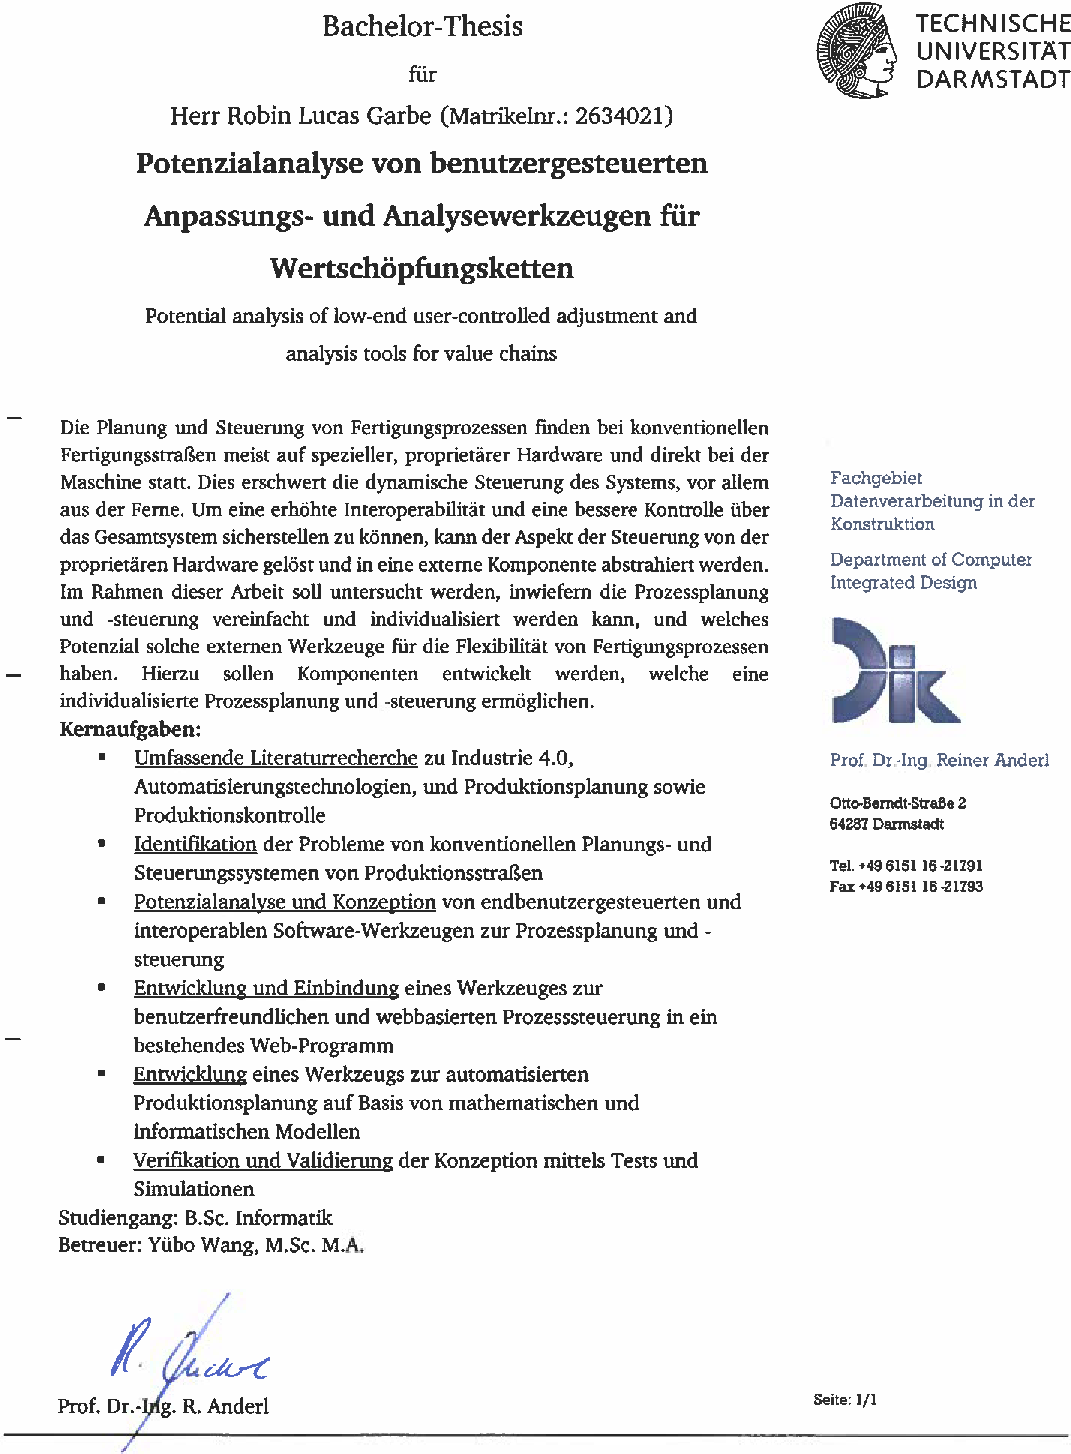
\includegraphics[width=1.007\textwidth]{images/01/Thema.pdf}\hspace{-1cm}\vspace{-3cm}
\end{figure}

% =================================================================================================== %
                                                                            % │ %
% ──────────────────────────────────────────────────────────────────────────────────────────────────┘ %


% ┌─────────────────────────────────────────────────────────────────────────────────────────────────┐ %
% │ Abstract einfügen                                                                             % │ %
% └─────────────────────────────────────────────────────────────────────────────────────────────────┤ %
\pdfbookmark[0]{Abstract}{abstract}                                                               % │ %
% =================================================================================================== %
% Abstract
% =================================================================================================== %
\hfill
\section*{Kurzfassung}
Seit nunmehr einigen Jahren ist ein zunehmendes Aufkommen von allgegenwärtigen Verknüpfungen mit digitalen Objekten unter dem Namen „Internet of Things“ (IoT; auch bekannt als Internet of Objects) zu bemerken. Historisch waren Industrial Automation and Control Systems (IACS, dt.: Industrielle Automations- und Kontrollsysteme) jedoch größtenteils von einer solchen Verknüpfung ausgenommen. Um diese Lücke zu schließen, ist in jüngerer Vergangenheit das Konzept des Industrial Internet of Things (IIoT) aufgekommen. Dessen Ziel ist es, eine industrielle Infrastruktur über ähnliche Methoden wie beim IoT anzubinden.

Diese Thesis beschäftigt sich mit dem daraus hervorgehenden Potenzial der endbenutzergesteuerten Prozesssteuerung, -analyse, und -planung, sowie mit den Herausforderungen, die dadurch entstehen. Dabei wird untersucht, inwiefern diese Aspekte vereinfacht und individualisiert werden können. Des Weiteren werden webbasierte und interoperable Software-Komponenten entwickelt, in eine Demonstrationsplattform eingebunden und analysiert.

\textbf{Schlüsselwörter:} Industrie 4.0, Industrial Internet of Things (IIoT), Prozesssteuerung, Produktionsplanung, REST, OPC-UA, Manufacturing Bill of Materials (MBOM)

%\vspace{15mm}
\newpage
\hfill

\selectlanguage{english}
\section*{Abstract}
For some years now, one has noticed an increasing emergence of ubiquitous connections with digital objects under the name „Internet of Things“ (IoT; also known as Internet of Objects). Historically, Industrial Automation and Control Systems (IACS) were largely excluded from such a link. To close this gap, the concept of the Industrial Internet of Things (IIoT) has recently emerged. It aims to connect an industrial infrastructure using methods similar to those used for the IoT.

This thesis deals with the resulting potential of end-user-controlled process control, analysis and planning, as well as with the challenges that arise from this. It is examined to what extent these aspects can be simplified and individualized. Furthermore, web-based and interoperable software components are developed, integrated into a demonstration platform, and analyzed.

\textbf{Keywords:} Industrie 4.0, Industrial Internet of Things (IIoT), Process Control, Production Planning, REST, OPC-UA, Manufacturing Bill of Materials (MBOM)
\selectlanguage{ngerman}
% =================================================================================================== %
                                                                         % │ %
% ──────────────────────────────────────────────────────────────────────────────────────────────────┘ %


% ─ ─ ─ ─ ─ ─ ─ ─ ─ ─ ─ ─ ─ ─ ─ ─ ─ ─ ─ ─ ─ ─ ─ ─ ─ ─ ─ ─ ─ ─ ─ ─ ─ ─ ─ ─ ─ ─ ─ ─ ─ ─ ─ ─ ─ ─ ─ ─ ─ ┐ %
\pagenumbering{roman}                                                                             % │ %
% ─ ─ ─ ─ ─ ─ ─ ─ ─ ─ ─ ─ ─ ─ ─ ─ ─ ─ ─ ─ ─ ─ ─ ─ ─ ─ ─ ─ ─ ─ ─ ─ ─ ─ ─ ─ ─ ─ ─ ─ ─ ─ ─ ─ ─ ─ ─ ─ ─ ┘ %


% ┌─────────────────────────────────────────────────────────────────────────────────────────────────┐ %
% │ Inhaltsverzeichnis                                                                            % │ %
% └─────────────────────────────────────────────────────────────────────────────────────────────────┤ %
\pdfbookmark[0]{Inhaltsverzeichnis}{toc}                                                          % │ %
\tableofcontents                                                                                  % │ %
\clearpage                                                                                        % │ %
% ──────────────────────────────────────────────────────────────────────────────────────────────────┘ %


% ┌─────────────────────────────────────────────────────────────────────────────────────────────────┐ %
% │ Abbildungsverzeichnis                                                                         % │ %
% └─────────────────────────────────────────────────────────────────────────────────────────────────┤ %
\pdfbookmark[0]{Abbildungsverzeichnis}{lof}                                                       % │ %
\listoffigures                                                                                    % │ %
\clearpage                                                                                        % │ %
% ──────────────────────────────────────────────────────────────────────────────────────────────────┘ %


% ┌─────────────────────────────────────────────────────────────────────────────────────────────────┐ %
% │ Tabellenverzeichnis                                                                           % │ %
% └─────────────────────────────────────────────────────────────────────────────────────────────────┤ %
\pdfbookmark[0]{Abbildungsverzeichnis}{lot}                                                       % │ %
\listoftables                                                                                     % │ %
\clearpage                                                                                        % │ %
% ──────────────────────────────────────────────────────────────────────────────────────────────────┘ %


% ┌─────────────────────────────────────────────────────────────────────────────────────────────────┐ %
% │ Symbole und Abkürzungen                                                                       % │ %
% └─────────────────────────────────────────────────────────────────────────────────────────────────┤ %
\pdfbookmark[0]{Symbole und Abkürzungen}{symbole}                                                 % │ %
%\chapter*{Symbole und Abkürzungen}
\chapter*{Abkürzungen}

% \section*{Symbole}
% \begin{tabular}{@{}l@{\qquad}l}
%   $I$ & Strom (A)\\
%   $R$ & Widerstand ($\Omega$)\\
%   $U$ & Spannung (V)\\
%   \\
%   $\sigma$     & Standardabweichung\\
%   $\omega$     & Kreisfrequenz ($1/\mathrm{s}$)
% \end{tabular}

%\section*{Abkürzungen}
\begin{tabular}{@{}l@{\qquad}l}
  API   & Application Programming Interface\\
  App   & Application\\
  AWS   & Amazon Web Services\\
  CPS   & Cyber-Physische Systeme\\
  ERP   & Enterprise Resource Planning\\
  HATEOAS & Hypermedia as the Engine of Application State\\
  HMI   & Human-Machine-Interface\\
  HTTP  & Hypertext Transfer Protocol\\
  HTTPS & Hypertext Transfer Protocol Secure\\
  IACS  & Industrial Automation and Control Systems\\
  IIC   & Industrial Internet Consortium\\
  IIoT  & Industrial Internet of Things\\
  IoS   & Internet of Services\\
  IoT   & Internet of Things\\
  IP    & Internet Protocol\\
  JSON  & JavaScript Object Notation\\
  JWT   & JavaScript Web Tokens\\
  KI    & Künstliche Intelligenz\\
  MaaS  & Manufacturing-as-a-Service\\
  MAC   & Media Access Control\\
  MBOM  & Manufacturing bill of materials\\
  MEMS  & Microelectromechanical Systems\\
  MQTT  & Message Queuing Telemetry Transport\\
  OPC   & Open Platform Communications\\
  OPC-UA & OPC Unified Architecture\\
  PLC   & Programmable Logic Controller\\
  Pub/Sub & Publish/Subscribe
\end{tabular}
\newpage
\begin{tabular}{@{}l@{\qquad}l}
  REST  & Representational State Transfer\\
  RFID  & Radio-frequency identification\\
  SCADA & Supervisory Control and Data Acquisition\\
  SPS   & Speicherprogrammierbare Steuerung\\
  TCP   & Transmission Control Protocol\\
  TLS   & Transport Layer Security\\
  TSN   & Time Sensitive Network\\
  URI   & Uniform Resource Identifier\\
  URL   & Uniform Resource Locator\\
  UUID  & Universally Unique Identifiers\\
  WAMP  & Web Application Messaging Protocol\\
  WASM  & WebAssembly\\
  WWW   & World Wide Web\\
  XML   & Extensible Markup Language
\end{tabular}
                                                                            % │ %
\clearpage                                                                                        % │ %
% ──────────────────────────────────────────────────────────────────────────────────────────────────┘ %


% ╔═════════════════════════════════════════════════════════════════════════════════════════════════╗ %
% ║ Hauptteil                                                                                     % ║ %
% ╚═════════════════════════════════════════════════════════════════════════════════════════════════╣ %
\pagenumbering{arabic}                                                                            % ║ %
\subimport*{chapters/01}{_Einleitung}                                                             % ║ %
\subimport*{chapters/02}{_Stand}                                                                  % ║ %
\subimport*{chapters/03}{_Grundlagen}                                                             % ║ %
\subimport*{chapters/04}{_Prozessplanung}                                                         % ║ %
\subimport*{chapters/05}{_Produktionsplanung}                                                     % ║ %
\subimport*{chapters/06}{_Verifikation}                                                           % ║ %
\subimport*{chapters/07}{_Ausblick}                                                               % ║ %
\clearpage                                                                                        % ║ %
% ══════════════════════════════════════════════════════════════════════════════════════════════════╝ %


% ─ ─ ─ ─ ─ ─ ─ ─ ─ ─ ─ ─ ─ ─ ─ ─ ─ ─ ─ ─ ─ ─ ─ ─ ─ ─ ─ ─ ─ ─ ─ ─ ─ ─ ─ ─ ─ ─ ─ ─ ─ ─ ─ ─ ─ ─ ─ ─ ─ ┐ %
\pagenumbering{roman}                                                                             % │ %
% ─ ─ ─ ─ ─ ─ ─ ─ ─ ─ ─ ─ ─ ─ ─ ─ ─ ─ ─ ─ ─ ─ ─ ─ ─ ─ ─ ─ ─ ─ ─ ─ ─ ─ ─ ─ ─ ─ ─ ─ ─ ─ ─ ─ ─ ─ ─ ─ ─ ┘ %


% ┌─────────────────────────────────────────────────────────────────────────────────────────────────┐ %
% │ Literaturverzeichnis                                                                          % │ %
% └─────────────────────────────────────────────────────────────────────────────────────────────────┤ %
\printbibliography                                                                                % │ %
% ──────────────────────────────────────────────────────────────────────────────────────────────────┘ %


% ┌─────────────────────────────────────────────────────────────────────────────────────────────────┐ %
% │ Anhang                                                                                        % │ %
% └─────────────────────────────────────────────────────────────────────────────────────────────────┤ %
\appendix                                                                                         % │ %
\chapter{Anhang}
\label{cha:anhang}

\begin{lstlisting}[language=XML,caption={XML Code für simplen Prozess},captionpos=b,label={lst:anhang_code_xml}]
<xml xmlns="https://developers.google.com/blockly/xml">
    <block type="PLC_Distribute_ExtendSlide__ON" id="w[,^tOV?1A2pYgamWghr" x="15" y="88">
        <next>
            <block type="instruction_wait" id="FFAUMYks/WAmp_I=ASlj">
                <field name="wait_amount">0.2</field>
                <next>
                    <block type="PLC_Distribute_ExtendSlide__OFF" id=".[Hx1gsNm1`I_?Epql~O">
                        <next>
                            <block type="PLC_Distribute_ConveyerForward__ON" id="6k8D(GT3vcFL96uzt3-+">
                                <next>
                                    <block type="instruction_wait" id="qi(*IulXH*3u9LH3,j`z">
                                        <field name="wait_amount">4.3</field>
                                        <next>
                                            <block type="PLC_Distribute_ConveyerForwa rd__OFF" id="1jdIM*0Nm(ulS29B3{LF"/>
                                        </next>
                                    </block>
                                </next>
                            </block>
                        </next>
                    </block>
                </next>
            </block>
        </next>
    </block>
</xml>
\end{lstlisting}

\begin{lstlisting}[language=JavaScript,caption={Code zur Erstellung des Prozess-Randdaten-Objektes},captionpos=b,label={lst:anhang_code_analyse}]
const allUsedActuatorsRaw = [...$(xml).find('block')]
		.map((el) => dic(el.getAttribute("type")))
		.filter((el) => el !== "instruction_wait");
const usedActuators = [...new Set([...$(xml).find('block')]
		.map((el) => dic(el.getAttribute("type").substring(0, el.getAttribute("type").indexOf("__"))))
		.filter((el) => el !== ""))];

const mbomAnalysis = {
    executionTime: Math.round([...$(xml).find('field[name="wait_amount"]')]
    		.map((el) => Number(el.textContent))
    		.reduce((sum, step) => sum + step)*100)/100,
	usedActuators: usedActuators,
	usedResources: [
		{
			name: "cup",
			amount: allUsedActuatorsRaw.filter((el) => el === "PLC_Distribute_ExtendSlide__ON").length
		},
		{
			name: "lid",
			amount: allUsedActuatorsRaw.filter((el) => el === "PLC_Distribute_Vacuum__ON").length
		}
	],
	nbrOfGroups: $(xml).children('block').length,
	nbrOfBlocks: $(xml).find('block').length
};
\end{lstlisting}
%
\begin{figure}[htbp]
	\centering\includegraphics[width=1.0\textwidth]{images/anhang/Screenshot_Prozessplanung.png}
    \caption{Ganzseitiger Screenshot der Prozessplanungs und -steuerungs Seite}
    \label{fig:anhang_Screenshot_Prozessplanung}
\end{figure}
%
\begin{figure}[htbp]
	\centering\includegraphics[width=1.0\textwidth]{images/anhang/Screenshot_Übersichtsseite.png}
    \caption{Ganzseitiger Screenshot der Übersichts-Seite}
    \label{fig:anhang_Screenshot_Übersichtsseite}
\end{figure}
%
\begin{figure}[htbp]
	\centering\includegraphics[width=1.0\textwidth]{images/anhang/Screenshot_Produktionsplanung.png}
    \caption{Ganzseitiger Screenshot der Produktionsplanungs-Seite}
    \label{fig:anhang_Screenshot_Produktionsplanung}
\end{figure}
                                                                             % │ %
% ──────────────────────────────────────────────────────────────────────────────────────────────────┘ %


% ╔═════════════════════════════════════════════════════════════════════════════════════════════════╗ %
% ║ Ende des Dokumentes                                                                           % ║ %
% ╚═════════════════════════════════════════════════════════════════════════════════════════════════╣ %
\end{document}                                                                                    % ║ %
% ══════════════════════════════════════════════════════════════════════════════════════════════════╝ %
